% Ass02: บันทึกการสำรวจไฟล์ .pkt ใน Cisco Packet Tracer
\section{สิ่งที่สังเกตได้จากการจำลอง}

\begin{figure}[h]
  \centering
  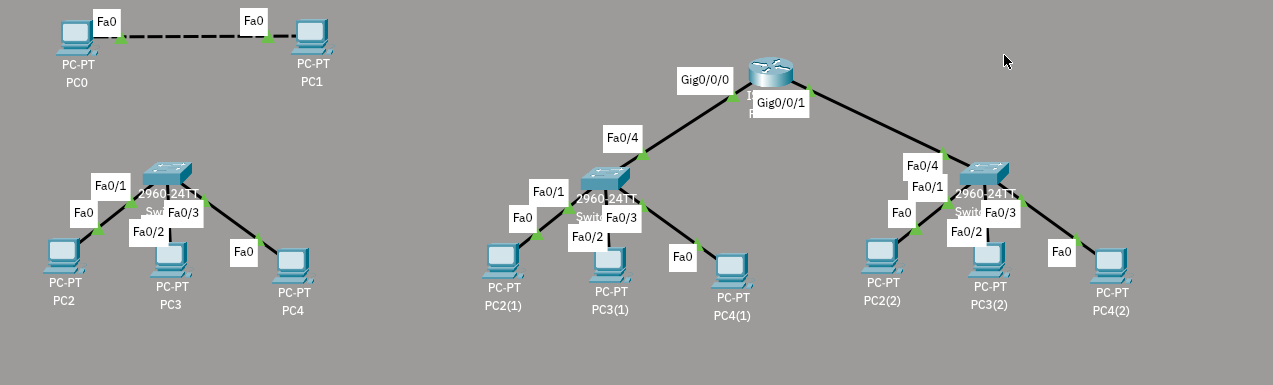
\includegraphics[width=\linewidth]{topology}
  \caption{Network Topology จากไฟล์ .pkt ใน Cisco Packet Tracer}
  \label{fig:topology}
\end{figure}

รูปที่~\ref{fig:topology} มีเครือข่าย 3 แบบ ได้แก่ PC0 กับ PC1 ที่ต่อสายถึงกันโดยตรง, PC2 ถึง PC4 ที่ต่อผ่าน Switch 2960 ตัวเดียว และอีกสองกลุ่มที่แต่ละกลุ่มมี Switch ของตัวเอง แล้ว Switch ทั้งสองต่อเข้ากับ Router ผ่านพอร์ต Gig0/0/0 และ Gig0/0/1

\subsection*{Host}
Host ทั้งหมดเป็น PC-PT จำนวน 11 เครื่อง แบ่งเป็น 4 วง: วง A มี PC0 และ PC1, วง B มี PC2 ถึง PC4, วง C มี PC2(1) ถึง PC4(1) และวง D มี PC2(2) ถึง PC4(2)

\subsection*{Network}
วง A ต่อสายตรงระหว่าง PC สองเครื่อง วง B ต่อ PC ทั้งสามเครื่องเข้ากับ Switch ตัวเดียว ส่วนวง C และวง D แต่ละวงมี Switch ของตัวเอง และ Switch ทั้งสองต่อขึ้นไปที่ Router ตัวเดียวกัน วง A, B และ C ใช้ช่วง 192.168.0.x เหมือนกัน แต่ไม่มีสายเชื่อมถึงกัน จึงใช้ IP ซ้ำกันได้โดยไม่ชนกัน

\subsection*{Router}
มี Router 1 ตัว (Router1) ใช้เชื่อมวง C (192.168.0.0/24) กับวง D (192.168.1.0/24) ซึ่งเป็นคนละ network กัน วง A และวง B ไม่มี Router

\subsection*{Interface}
PC ทุกเครื่องใช้พอร์ต Fa0 ส่วน Switch 2960 ทุกตัวต่อ PC ที่พอร์ต Fa0/1 ถึง Fa0/3 สำหรับวง C และ D ใช้พอร์ต Fa0/4 ต่อขึ้น Router ที่พอร์ต Gig0/0/0 (วง C) และ Gig0/0/1 (วง D) Switch ไม่มี IP ของตัวเอง (Vlan1 อยู่ในสถานะ down)

\subsection*{IP Address, Network Mask และ Default Gateway}
ทุกวงใช้ Network Mask 255.255.255.0 (/24) ดูค่าของแต่ละอุปกรณ์ได้ในตารางที่~\ref{tab:ip}

\begin{table}[h]
  \centering
  \caption{IP Address และ Default Gateway ของแต่ละอุปกรณ์}
  \label{tab:ip}
  \begin{tabular}{cllll}
    \toprule
    วง & อุปกรณ์ & พอร์ต & IP Address & Default Gateway \\
    \midrule
    A & PC0     & Fa0      & 192.168.0.1 & ไม่มี \\
    A & PC1     & Fa0      & 192.168.0.2 & ไม่มี \\
    \midrule
    B & PC2     & Fa0      & 192.168.0.1 & ไม่มี \\
    B & PC3     & Fa0      & 192.168.0.2 & ไม่มี \\
    B & PC4     & Fa0      & 192.168.0.3 & ไม่มี \\
    \midrule
    C & Router1 & Gig0/0/0 & 192.168.0.1 & (เป็น gateway ของวง) \\
    C & PC2(1)  & Fa0      & 192.168.0.2 & 192.168.0.1 \\
    C & PC3(1)  & Fa0      & 192.168.0.3 & 192.168.0.1 \\
    C & PC4(1)  & Fa0      & 192.168.0.4 & 192.168.0.1 \\
    \midrule
    D & Router1 & Gig0/0/1 & 192.168.1.1 & (เป็น gateway ของวง) \\
    D & PC2(2)  & Fa0      & 192.168.1.2 & 192.168.1.1 \\
    D & PC3(2)  & Fa0      & 192.168.1.3 & 192.168.1.1 \\
    D & PC4(2)  & Fa0      & 192.168.1.4 & 192.168.1.1 \\
    \bottomrule
  \end{tabular}
\end{table}

วง A และวง B ไม่มี Router จึงไม่ต้องตั้ง Default Gateway ส่วน PC ในวง C และวง D ใช้ IP ของพอร์ต Router ฝั่งเดียวกันเป็น Default Gateway

\section{คำถาม}

\subsection*{1. What is the smallest network? (เครือข่ายที่เล็กที่สุดคืออะไร?)}
เครือข่ายที่เล็กที่สุดคือวง A ซึ่งมี PC แค่ 2 เครื่อง (PC0 กับ PC1) ต่อสายตรงจาก Fa0 ถึง Fa0 โดยไม่ใช้ Switch หรือ Router

\subsection*{2. What network requires switches? (เครือข่ายลักษณะใดจำเป็นต้องใช้ Switch?)}
เครือข่ายที่มี Host มากกว่า 2 เครื่องใน network เดียวกัน เพราะ PC แต่ละเครื่องมีพอร์ต Fa0 แค่พอร์ตเดียว เช่น วง B ที่ PC2, PC3 และ PC4 ต่อเข้า Switch 2960 ที่พอร์ต Fa0/1 ถึง Fa0/3

\subsection*{3. What network requires routers? (เครือข่ายลักษณะใดจำเป็นต้องใช้ Router?)}
เครือข่ายที่ต้องเชื่อมคนละ network เข้าด้วยกัน เช่น วง C (192.168.0.x) กับวง D (192.168.1.x) ที่ Router1 เชื่อมไว้ผ่านพอร์ต Gig0/0/0 และ Gig0/0/1 โดย Switch แต่ละตัวต่อขึ้น Router ที่พอร์ต Fa0/4
